% This is a simple sample document.  For more complicated documents take a look in the exercise tab. Note that everything that comes after a % symbol is treated as comment and ignored when the code is compiled.

\documentclass{article} % \documentclass{} is the first command in any LaTeX code.  It is used to define what kind of document you are creating such as an article or a book, and begins the document preamble

\usepackage{amsmath} % \usepackage is a command that allows you to add functionality to your LaTeX code
\usepackage{graphicx}
\usepackage{wrapfig}
\usepackage{tabularx}
\usepackage{caption}
\usepackage[utf8]{inputenc}


\title{Obliczenia Naukowe Lista 3} % Sets article title
\author{Szymon Pestrowicz} % Sets authors name
\date{\today} % Sets date for date compiled

% The preamble ends with the command \begin{document}
\begin{document} % All begin commands must be paired with an end command somewhere
	\maketitle % creates title using information in preamble (title, author, date)

	\section*{Zadanie 1} % creates a section

		W pierwszym zadaniu należy napisać funkcje obliczajaca ilorazy różnicowe czyli inaczej przyrost funkcji na danym przedziale na podstawie wektora x (wezły) oraz wektora f (wartości) bez użycia tablicy dwuwymiarowej (macierzy). Funkcja zaimplementowana przeze mnie korzysta z takiego wzoru: $f(x_i) = \frac{f(x_i) - f(x_{i-1})}{x_i - x_{i-1}}$


	\section*{Zadanie 2} % creates a section

		W drugim zadaniu należy napisać funkcje obliczajaca wartość wielomianu interpolacyjnego stopnia n w postaci Newtona $N_n(x)$ w punkcie $x=t$ przy użyciu algorytmu hornera. Dane wejsciowe funkcji : x (wezły), fx (ilorazy różnicowe), t (punkt w którym należy obliczyć wartość wielomianu). Koncepcja algorytmu hornera: $W(x) = a_0 + a_1x+a_2x^2+...+a_{n-1}x^{n-1}+a_nx^n$ można przekształcić na $W(x) = a_0 + x(a_1 + x(a_2 + ... + x)a_{n-1} + xa_n)...))$

	\section*{Zadanie 3} % creates a section
		
		W trzecim zadaniu należy napisać funkcje obliczajaca współczynniki postaci naturalnej wielomianu na podstawie x (wezłów) oraz oraz fx (ilorazów różnicowych). Do obliczania używam wzoru z wykładu na postać  Newtona: \\$\sum_{k=0}^{n} f[x_0,x_1,...,x_k]\prod_{j=0}^{k-1}(x-x_j)$

	\section*{Zadanie 4} % creates a section
		
		W czwartym zadaniu należy napisać funkcje która zinterpoluje zadana funkcje $f(x)$ w przedziale $[a,b]$ za pomoca wielomianu interpolacyjnego stopania n w postaci Newtona a nastepnie narysuje ten wielomian interpolacyjny i interpolowana funkcje. Oto przykładowy wykres dla funkcji $|x|$ w przedziale $[-1.0;1.0]$ oraz dla stopnia wielomianu interpolacyjnego $= 5$
		
		\begin{figure}
		 	\begin{minipage}{1.0\textwidth}
   				\centering
   				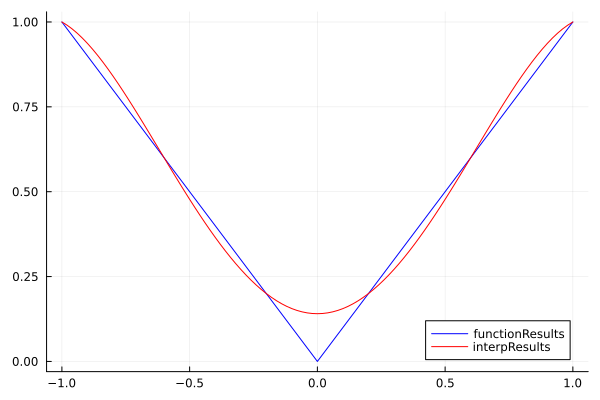
\includegraphics[width=0.9\linewidth]{4.png}
   				\caption*{$|x|$}
 			\end{minipage}%
		\end{figure}

	\section*{Zadanie 5} % creates a section
		
		Zadanie 5 polega na przeterstowaniu funkcji z zadania 4 na nastepujacych przykładach:

		$e^x$ na przedziale $[0;1.0]$ oraz na stopniach wielomianu podanych pod każdym wykresem.

		\begin{figure}[h]
		 	\begin{minipage}{0.33\textwidth}
   				\centering
   				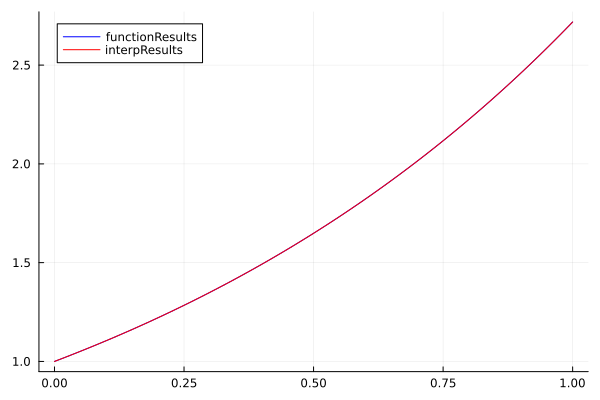
\includegraphics[width=0.9\linewidth]{5a5.png}
   				\caption*{$5$}
 			\end{minipage}%
			\begin{minipage}{0.33\textwidth}
   				\centering
   				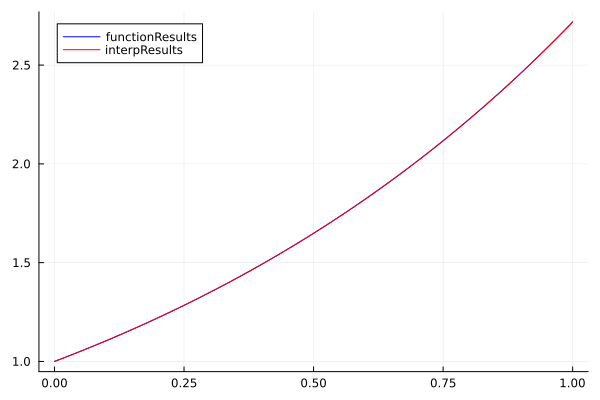
\includegraphics[width=0.9\linewidth]{5a10.png}
   				\caption*{$10$}
 			\end{minipage}%
			\begin{minipage}{0.33\textwidth}
   				\centering
   				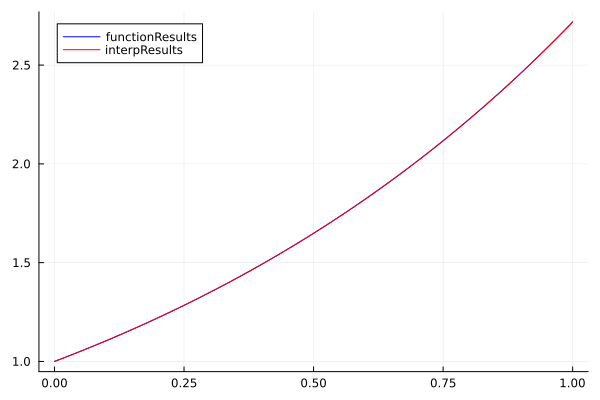
\includegraphics[width=0.9\linewidth]{5a15.png}
   				\caption*{$15$}
 			\end{minipage}%
		\end{figure}
		\vspace{5.0cm}

		$x^2sin(x)$ na przedziale $[-1.0;1.0]$ oraz na stopniach wielomianu podanych pod każdym wykresem.

		\begin{figure}[h]
		 	\begin{minipage}{0.33\textwidth}
   				\centering
   				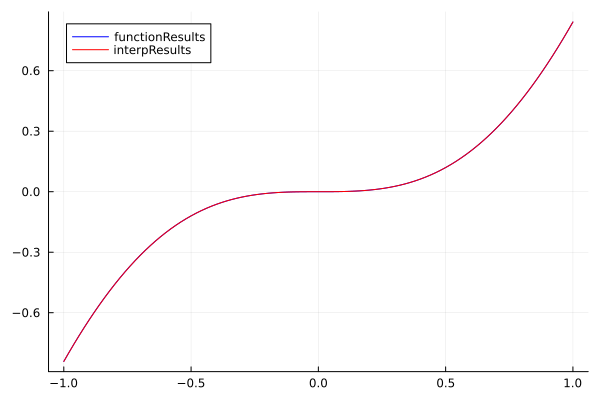
\includegraphics[width=0.9\linewidth]{5b5.png}
   				\caption*{$5$}
 			\end{minipage}%
			\begin{minipage}{0.33\textwidth}
   				\centering
   				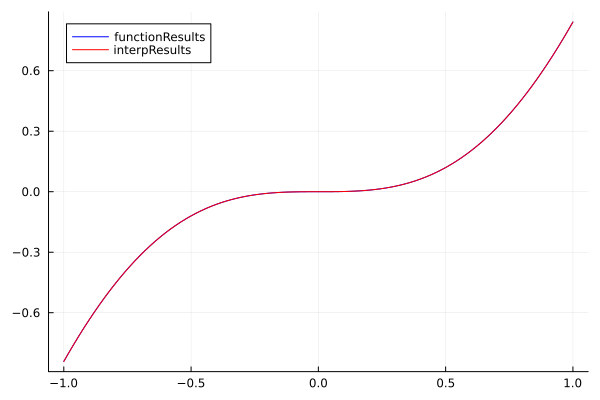
\includegraphics[width=0.9\linewidth]{5b10.png}
   				\caption*{$10$}
 			\end{minipage}%
			\begin{minipage}{0.33\textwidth}
   				\centering
   				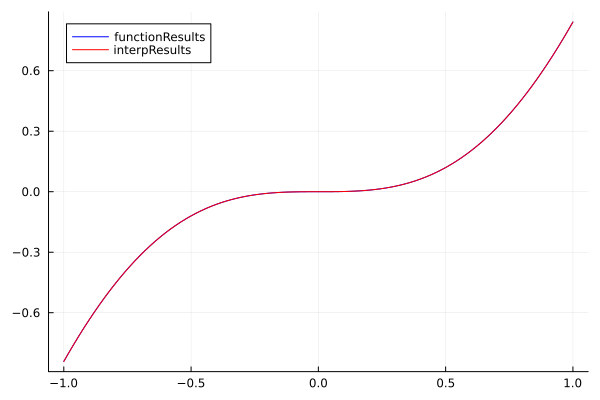
\includegraphics[width=0.9\linewidth]{5b15.png}
   				\caption*{$15$}
 			\end{minipage}%
		\end{figure}

	\section*{Zadanie 6} % creates a section
		
		Zadanie 6 polega na przeterstowaniu funkcji z zadania 4 na nastepujacych przykładach:

		$|x|$ na przedziale $[-1.0;1.0]$ oraz na stopniach wielomianu podanych pod każdym wykresem.

		\begin{figure}[h]
		 	\begin{minipage}{0.33\textwidth}
   				\centering
   				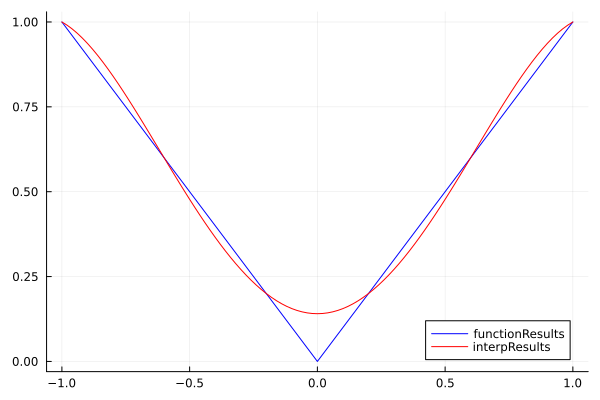
\includegraphics[width=0.9\linewidth]{6a5.png}
   				\caption*{$5$}
 			\end{minipage}%
			\begin{minipage}{0.33\textwidth}
   				\centering
   				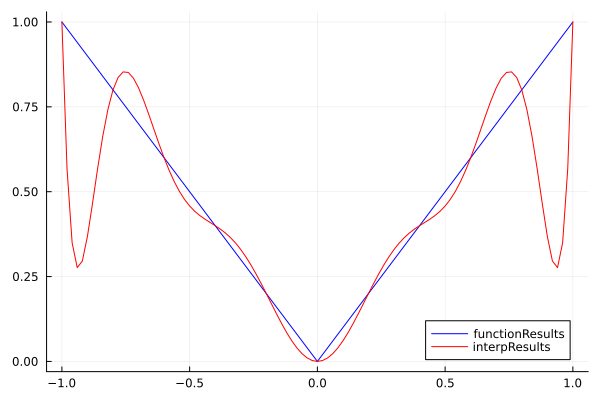
\includegraphics[width=0.9\linewidth]{6a10.png}
   				\caption*{$10$}
 			\end{minipage}%
			\begin{minipage}{0.33\textwidth}
   				\centering
   				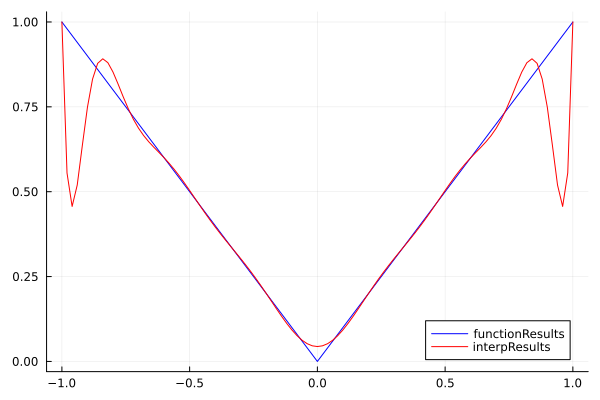
\includegraphics[width=0.9\linewidth]{6a15.png}
   				\caption*{$15$}
 			\end{minipage}%
		\end{figure}

		$\frac{1}{1+x^2}$ na przedziale $[-5.0;5.0]$ oraz na stopniach wielomianu podanych pod każdym wykresem.

		\begin{figure}[h]
		 	\begin{minipage}{0.33\textwidth}
   				\centering
   				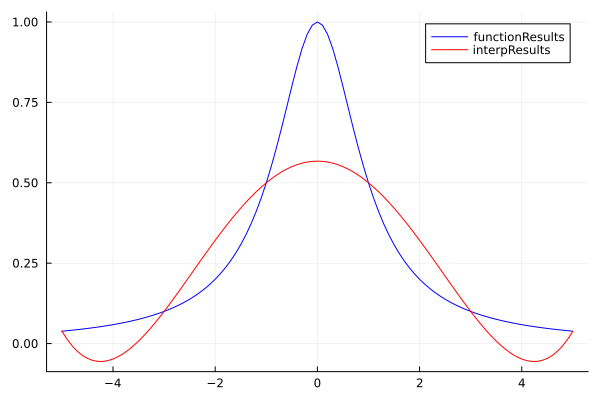
\includegraphics[width=0.9\linewidth]{6b5.png}
   				\caption*{$5$}
 			\end{minipage}%
			\begin{minipage}{0.33\textwidth}
   				\centering
   				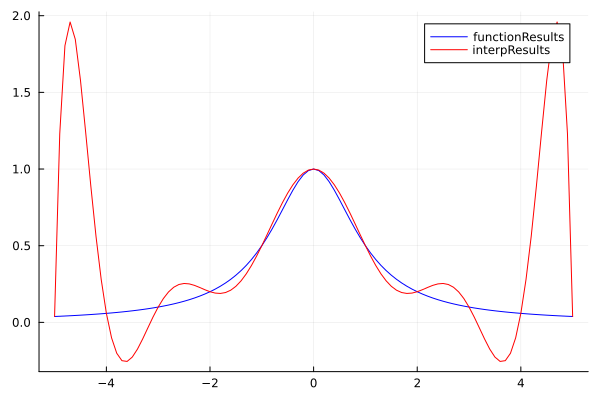
\includegraphics[width=0.9\linewidth]{6b10.png}
   				\caption*{$10$}
 			\end{minipage}%
			\begin{minipage}{0.33\textwidth}
   				\centering
   				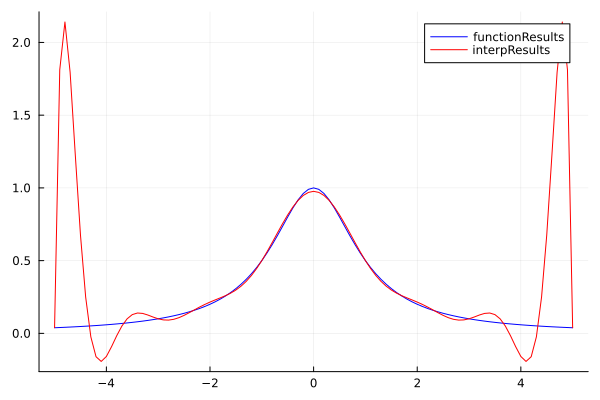
\includegraphics[width=0.9\linewidth]{6b15.png}
   				\caption*{$15$}
 			\end{minipage}%
		\end{figure}

		W zadaniu 6 na pierwszy rzut oka widać, że wykresy nie pokrywaja sie tak jak w zadaniu 5. Jest to zjawisko Runge'go, czyli pogorszenie jakości interpolacji wielomianowej, mimo zwiekszenia liczby jej wezłów. Poczatkowo ze wzrostem liczby wezłów n przybliżenie poprawia sie, jednak po dalszym wzroście n, zaczyna sie pogarszać, co jest szczególnie widoczne na końcach przedziałów. Takie zachowanie sie wielomianu interpolujacego jest zjawiskiem typowym dla interpolacji za pomoca wielomianów wysokich stopni przy stałych odległościach wezłów. Wystepuje ono również, jeśli interpolowana funkcja jest nieciagła albo odbiega znaczaco od funkcji gładkiej. Aby uniknać tego efektu, stosuje sie interpolacje z wezłami coraz geściej upakowanymi na krańcach przedziału interpolacji.

\end{document} % This is the end of the document